\mychapter{Multi Issuer Multi Credential Anonymous Credentials (MIMC-ABC)}\label{sec:mimc}

Motivate MIMCABC

Problems: 
1. How can users privately combine credentials from multiple, mutually distrusting issuers (e.g., government IDs and bank statements) to prove they belong to the same identity?

2. How to improve the accountability of that process

Use Cases (Where this is needed)
- User is presenting their portfolio of images which have been digitally signed by different cameras, the user was logged in to the cameras with their account/identifier. 
The issuer is the camera, the verifier is the website. 
The commitment holds the user identifier and content hash. 
The user proves identity binding across credentials and selectively discloses the content hash.
(an app could be a user takes photos, each photo is signed by the phone, the signer has the user id and content hash)

- Anonymous Payment Systems like UTT




















Multi-Issuer Multi-Credential System (MIMC-ABC) (Chapter 3)
– Formalized security model for multi-issuer identity binding with position-binding commit-
ments
– Proved unforgeability and anonymity even against colluding credential issuers
– Demonstrated 30\% performance improvement over comparable schemes for multi-credential
verification


Chapter 3: Multi-Issuer Multi-Credential System: How can users privately combine credentials from multiple, mutually distrusting issuers (e.g., government IDs and bank statements) to prove they belong to the same identity? Non-private systems easily verify credential consistency, but privacy-preserving approaches struggle to bind credentials securely without
a trusted party, aggregate signatures [MBG+23] have trouble with revoking individual credentials from an aggregate.
Technical Challenges
1. Defining and achieving identity binding across credentials without revealing the user’s identity.
2. Preventing attacks where users mix credentials from different identities (e.g., credential swapping).
3. Maintaining efficiency as the number of issuers and credentials scales

Some notes
- There are many credential oracles, ZK TLS, DECO, etc, ZK Login, all these products bring solid credentials or others into the web e.g. bank account details, statements, etc. We need a way to attach them to a users identifier and allow a user to use them AND prove that they belong to them. 
- I thought identity binding is a good way to do that, during the issuance process, the user gives a commitment to the identity, the issuer fills it in with their private information? or something like that, I'm not sure how ZK TLS or attested information oracles work.
- Also for different digital identity issuers





















\subsection{Notation}
We base our Multi Issuer, Multi Credential Multi-show Attribute based Anonymous Credentials off the model in \cite{fuchsbauer_structure-preserving_2019} and extend it to support rerandomizable signatures over commitments and predicate-based zero-knowledge proof verification allowing users to prove statements about their committed and signed attributes without revealing any additional information.

\subsection{Syntax}
\begin{definition}[MIMC-ABC System] A Multi-Issuer Multi-Credential Attribute-based Anonymous Credential system consists of the following $\PPT$ algorithms:
    \begin{itemize}
    \item $\mathsf{Setup}(\secparam) \to (\ppar)$ Takes security parameter $\lambda$ in unary, outputs public parameters $\ppar$.
    
    \item $\mathsf{OrgKeygen}(\ppar, \ell) \to (\osk, \opk)$: Is a probabilistic algorithm that takes public parameters $\ppar$ and $\ell$ the upper bound of credential attributes. Outputs organisation's keypair $(\osk, \opk)$
       
    \item $(\mathsf{Obtain}(\vec{m}, \opk, \aux), \mathsf{Issue}(\osk, \cm, \aux)) \rightarrow (\cred, \bot)$ is an interactive protocol between a user and an issuing organization. The user inputs their message vector $\vec{m} = [\id, \ctx, \attrs]$ containing a unique identifier $\id$ and context $\ctx$. User generates $\usk \sample Z_p$, commits to their messages $\cm \gets \CMCom(\vec{m}; \usk)$. The issuer inputs their secret key $\osk$. The protocol outputs a credential $\cred$ containing $(\sigma, \cm)$ to the user and $\bot$ to the issuer.    
    
    \item $(\mathsf{Show}(\{\credi\}, \{\uski\}, \phi), \mathsf{Verify}(\{\credi'\}, \pi)) \rightarrow \{0,1\}$ is an interactive protocol between a user and verifier. The user runs $\mathsf{Show}$ with their credentials (signatures and paired commitments), and secret keys. The user rerandomizes their credentials and commitments and computes a proof $\pi$ that satisfies the predicate $\phi$.
    $\Verify$ is run by the verifier, which takes input from the randomized credentials $\cred_i'$, randomized commitments $\cmi'$, and predicate, proof pair $\phi, \pi$. The protocol outputs 1 if verification succeeds, 0 otherwise.
    \end{itemize}
\end{definition}

\newpage
\subsection{Security Model}
% Intuition of our security. 

% Here i Can talk about the different attack vectors and how the security of our system changes between single issuer, single credential, to multi credential to multiple issuer.

\subsubsection{Security Properties}

\begin{itemize}
    \item Correctness ensures an honest user with valid credentials can always generate a proof for any predicate their credentials satisfy which will verify with high probability

    \item Unforgeability prevents a malicious user, or colluding users, from creating valid proof for new forged credentials, misuse of legitimately issued ones, or unauthorized combination of credentials they don't own.

    \item Anonymity protects user privacy, ensuring proofs reveal only that the predicate is satisfied, even if adversaries control the issuers or define predicates. 
\end{itemize}

To model the adversary’s capabilities and the system’s state, we introduce the following lists and oracles:


\noindent\textbf{Lists}
\begin{itemize}
    \item $\HU$: The set of honest users whose secret keys remain unknown to the adversary $\adv$
    \item $\CU$: The set of corrupt users whose secret keys are known to the adversary $\adv$
    \item $\CRED_j$: A list tracking all credentials issued by issuer $j$, where each credential is associated with a user and their attributes
    \item $\OWNR$: A mapping from each credential to its owning user, i.e., $\OWNR[\cred] = i$ if credential $\cred$ belongs to user $i$
    \item $\SHOW$: A list tracking all credential show outputs (\{\})
\end{itemize} 

\noindent\textbf{Oracles}
\begin{itemize}
    \item $\OHU()$: Creates a new honest user $i$, adds them to $\HU$, and returns $i$
    \item $\OCU(i)$: Corrupts user $i$ by moving them from $\HU$ to $\CU$, revealing their secret keys (e.g., commitment openings) and all credentials ${\cred}$ owned by $i$
    \item $\OOBTAIN(i, j, \vec{m})$: Issues a credential $\cred$ from issuer $j$ to user $i$ for the attribute vector $\vec{m}$, provided $i \in \HU$. The credential is added to $\CRED_j$, and $\OWNR[\cred]$ is set to $i$
    \item $\OSHOW(i, \phi)$: Generates a proof $\pi$ that the credentials of user $i$ satisfy the predicate $\phi$, provided $i \in \HU$ and the credentials meet the condition $\phi$. $\SHOW \cup \SHOW \{i, \pi\}$
\end{itemize} 



\begin{definition}[Correctness]
    \[
        \Pr \left[ 
            \Verify(\{\cred_k'\}, \{\cm_k'\}, \phi, \pi) = 1 \mid \text{all steps honest} \wedge \phi(\{m_k\}) = 1
        \right] = 1 - \negl[\lambda]
    \]
\end{definition}

\paragraph{Intuition:} A MIMC-ABC system is correct if, when all parties follow the protocol honestly, a user can successfully prove a true statement about their credentials to a verifier. Specifically, for all honestly generated public parameters, keys, credentials, and predicates satisfied by the user’s attributes, the verification process accepts the proof with overwhelming probability. 

    \begin{itemize}
        \item \textbf{Setup:} Challenger $\AdvC$ runs $\Setup(\secparam) \to \ppar$
        \item \textbf{Issuer Keys:} For each issuer $j$ in a set of issuers $\{j\}$, run $\OrgKeyGen(\ppar, \ell) \to (\osk_j, \opk_j)$.
        \item \textbf{Credential Issuance: } For a set of message vectors $\{m_k\}$, each $m_k = [\id, \ctx, \attrs, \usk_k]$ with the same $\id$. User runs $\UserKeyGen(\ppar) \to \usk_k$ and $\Obtain(\ppar, \opk_j, m_k, \aux),\Issue(\osk_j, \cm_k, \aux) \to \{\cred_k\}$. 
        \item \textbf{Proof Generation:} User runs $\Show(\{\cred_k'\}, \{\cm_k'\}, \phi, \pi)$ where $\{\cred_k'\}$ and $\{\cm_k'\}$ are rerandomized credentials and commitments.
        \item \textbf{Winning Condition:} Correctness holds if $\Verify(\{\cred_k'\}, \{\cm_k'\}, \phi, \pi) = 1 $ with $\Pr = 1-\negl[\lambda]$
    \end{itemize}
More formally,















\begin{definition}[Unforgeability]
A MIMC-ABC system is unforgeable if for all PPT adversaries $\mathcal{A}$, there exists a negligible function $\negl$ such that:
\[
\mathsf{Adv}\left[\mathrm{Game}^{\mathsf{\UNF}}_{\MIMCABC, \adv}(\lambda) = 1\right] \leq \negl[\secparam]
\]
\end{definition}

\paragraph{Intuition:} A MIMC-ABC system is unforgeable if no probabilistic polynomial-time (PPT) adversary can produce a valid proof for a predicate that they cannot legitimately satisfy, based on the credentials they have obtained or corrupted. This prevents \emph{forging credentials} or \emph{proving false statements} about them including faking identity binding and credential relationships when stated by $\phi$.

\paragraph{The intuition for the forgery success condition}: The adversary's forgery is successful if their proof verifies correctly \emph{and} the credentials used in the forgery cannot be traced back to a single corrupted user. The trivial forgery is one where the adversary corrupts a user and verifies a statement with their legitimately issued credentials. The adversary can win by combining credentials from multiple corrupt users to create valid proofs, combining credentials from corrupt users with newly forged credentials, and lastly creating entirely forged credentials. This is where our security properties, Identity Binding, and Credential Relationship Binding stem from.

\begin{remark}
    For \emph{identity binding}, if $\phi^*$ requires all $\id$ to match, $\AdvA$ can't mix credentials from different $\id$'s. For \emph{credential relationship binding}, if $\phi^*$ requires a specific relationship, for example $\cred_1$ contains $\CMCom([\id, \ctx="passport", \attrs]) \wedge \cred_2$ contains $\CMCom([\id, \ctx="driversLicense", \attrs])$ then $\AdvA$ can't win with different $\ctx$ or use something in $\attrs$ to satisfy $\phi^*$
    
\end{remark}



\begin{definition}[MIMC-ABC Anonymity]
A MIMC-ABC system provides anonymity if, for all PPT adversaries $\adv$, the advantage in the following experiment is negligible:
\[
\mathsf{Adv}^{\mathsf{anon}}_{\adv}(\secparam) = \left| \Pr[\mathrm{Game}^{\mathsf{anon-1}}_{\MIMCABC, \adv}(\secparam) = 1] - \Pr[\mathrm{Game}^{\mathsf{anon-0}}_{\MIMCABC, \adv}(\secparam) = 1] \right| \leq \negl(\lambda)
\]
\end{definition}

\begin{figure}
    \centering
    \begin{pcvstack}[boxed, center, space=1em]
        \begin{pchstack}
                 \begin{pcvstack}
                 \procedure[linenumbering]{$\mathrm{Game}^{\mathsf{\UNF}}_{\MIMCABC, \adv}(\secparam)$}{%
                    \pccomment{Challenger Setup} \\
                    \text{Initialize } \HU \gets \emptyset, \CU \gets \emptyset, \\
                    \CRED_j \gets \emptyset \text{ for each $j$}, \OWNR \gets \{\} \\
                    \ppar \gets \Setup(\secparam), (\osk_j, \opk_j) \gets \OrgKeyGen(\ppar) \\
                    \pccomment{$\AdvA$ queries oracles} \\
                    \AdvA^{\OHU, \OCU, \OOBTAIN}(\opk_j) \\
                    \pccomment{Forgery} \\
                    \AdvA \text{ outputs } (\{\cred_k'^*\} = (\{\sigma_k'^*, \cm_k'^*\}) ) \\
                    \pccomment{Winning Condition} \\
                    \Verify(\{\cred_k'^*\}, \phi^*, \pi^*, \{\opk_j\}) = 1 \; \wedge \\
                    \t \forall k, \OWNR[\{\cred_k'^*\}] \neq i \in \CU \quad \pclinecomment{Version 1}\\
                    \t \nexists i \in \CU : \phi^*(\vec{m}_{i,k}) = 1 \quad \pclinecomment{Version 2}\\
                    \pccomment{i.e. the set of all $\{\cred_k'^*\}$} \\
                    \pccomment{cannot belong to the same corrupt user}
                }
            \end{pcvstack}
             \begin{pcvstack}
             \procedure[linenumbering]{$\mathrm{Game}^{\mathsf{\ANON}}_{\MIMCABC, \adv}(\lambda)$}{%
                    \ppar \gets \Setup(\secparam), \HU, \gets \emptyset, \CU \gets \emptyset \quad \pclinecomment{Challenger $\AdvC$ Setup} \\
                    \{\osk_j, \opk_j\} \gets \AdvA(\OrgKeyGen(\ppar)) \text{ for each issuer $j$}. \\
                    \text{For $i$ in } \bit: \qquad \pclinecomment{$\AdvC$ initializes two honest users }\\
                    \t \usk_i \gets \UserKeyGen(\ppar), \HU \gets \HU \cup \{i\}, \\
                    \t \quad i \text{ has } \vec{m} \text{ such that } \phi(\vec{m}) = 1 \\
                    \t \cm_i \gets \CMCom(\vec{m}_i; \usk_i),  \cred_i \gets \Issue(\osk, \cm_i) \\
                    \AdvA^{\OHU, \OCU, \OOBTAIN, \OSHOW}(\{\osk_j, \opk_j\} ) \qquad \pclinecomment{Learning Phase} \\
                    (i_0, i_1, \phi) \gets \AdvA() \qquad \pclinecomment{Challenge Phase}\\
                    \text{Assert } i_0, i_1 \in \HU \setminus \CU, \quad \wedge \quad \phi(\vec{m}_{i_0}) = 1, \phi(\vec{m}_{i_1}) = 1 \\
                    b \sample \bit \quad \pclinecomment{$\AdvC$ samples random bit}\\
                    (\cred', \cm', \pi) \gets \Show(\creds_{i_b}, \cm_{i_b}, \usk_{i_b}, \phi)\\
                    b' \gets \AdvA(\cred', \cm', \pi) \qquad \pclinecomment{$\AdvA$ guesses who's $\cred$ it is } \\
                    \text{Return } b', \pclinecomment{Return the adversary guess}}
            \end{pcvstack}
        \end{pchstack}
        \end{pcvstack}
    \caption{Caption}
    % 
\end{figure}

\begin{figure}
    \centering
\begin{pchstack}[boxed]
        \begin{pcvstack}
            \procedure[]{$\OHU()$}{%
                \pcif i \notin \HU \cup \CU \\
                \t \HU \gets \HU \cup \{i\} \\
                \pcreturn  i \\
            }
            \procedure[]{$\OCU(i)$}{%
                \pcif i \in \HU:\\
                \t \HU \gets \HU \setminus \{i\} \\
                \t \CU \gets \CU \cup \{i\} \\
                \t \creds_i \gets \{\cred | \OWNR[\cred] = i\} \\
                \t \pcreturn \{(\cred, \usk) | (\cred, \cm, \vec{m}, \usk, i, j) \in \CRED\}\\
                \pcreturn \bot \\
            }
        \end{pcvstack}
        \begin{pcvstack}
            \procedure[]{$\OOBTAIN(i, j, \vec{m})$}{%
                \pcif i \in \HU: \\
                \t \usk \sample \Z_p \\
                \t \cm \gets \CMCom([\vec{m}]; \usk) \\
                \t \cred \gets \Issue(\osk_j, \cm) \\
                \t \CRED \gets (\cred, \cm, \vec{m}, \usk, i, j), \\
                \t \OWNR[\cred] = i \\
                \pcreturn \cred \\
            }
            \procedure[]{$\OSHOW(i, \creds_i, \phi)$}{%
                \pcif i \in \HU \; \wedge \; \phi(\creds_i) = 1: \\
                \t \text{Parse } \creds = \{\sigma, \cm, \vec{m}, \usk \} \\
                \t \pi \gets \Show(\creds_i, \phi) \\
                \t \pcreturn \pi \\
                \pcreturn \bot \\
            }
        \end{pcvstack}
    \end{pchstack}
    \caption{Caption}
    \label{}
\end{figure}


\paragraph{Anonymity: }A MIMC-ABC system provides anonymity if no PPT adversary can determine which user’s credentials were used in a proof, even if the adversary controls the issuers and chooses the messages and predicates. This ensures that presentations reveal only what the predicate explicitly requires, protecting user privacy.

\paragraph{Intuition}: the challenger sets up the game by picking a random bit $b \sample \bit$, which decides whether it uses "Alice or Bob's" credential in the game. Based on the bit, the challenger generates a credential "show" proof and presents it to the adversary. The adversary's guess should be no better than guessing.


























\newpage
\section{Construction}

\subsection{Intuition of Construction}

\subsubsection{Example}
Consider a user holding credentials from three issuers, denoted $j = 1, 2, 3$, each providing one credential $k = 1$. The user rerandomizes each credential’s commitment and signature as follows: $\cm_{j,1}' \gets \CMRand(\cm_{j,1}, \Delta_{r_{j,1}})$ and $\sigma_{j,1}' \gets \RSRand(\sigma_{j,1}, \Delta_{r_{j,1}}, \Delta_{u_{j,1}})$. These rerandomized pairs $(\cm_{j,1}', \sigma_{j,1}')$ are indistinguishable from their original issuance. In the $\Show$ protocol, the verifier confirms their validity: $\RSVer(\sigma_{j,1}', \cm_{j,1}', \vk_j) = 1$ for all $j \in \{1, 2, 3\}$.

\begin{figure}
        \begin{pchstack}[boxed, center, space=4em]
            \begin{pcvstack}
                \procedure[space=auto]{Passport}{%
                \id: 12345, \\
                \ctx: "passport", \\
                \attrs: \mathsf{values}
                }
            \end{pcvstack}
            \pcvspace
            \begin{pcvstack}
                \procedure[space=auto]{Driver License}{%
                 \id: 12345, \\
                \ctx: "dmv", \\
                 \attrs: \mathsf{values}
                }
            \end{pcvstack}
            \pcvspace
            \begin{pcvstack}
                \procedure[space=auto]{University Degree}{%
                 \id: 12345, \\
                \ctx: "usyd{-}bcompsc", \\
                \attrs: \mathsf{values}
                }
            \end{pcvstack}
        \end{pchstack}
    \caption{Three Example Credentials, $\attrs$ holds arbitrary number of attributes such as expiry}
    \label{fig:three-creds}
\end{figure}

Next, the user proves a relation $\mathcal{R}_\phi$ that ensures the credentials satisfy a predicate $\phi$. 
\[
\mathcal{R}_\phi = \left\{ 
\begin{array}{l} 
\forall j, k: \RSVer(\sigma_{j,k}', \cm_{j,k}', \vk_j) = 1 \\ 
\forall j, k: \cm_{j,k}' = \CMRand(\CMCom([\id, \ctx_{j,k}, \attrs_{j,k}]; \usk_{j,k}), \Delta_{r_{j,k}}) \\ 
\phi(\{\ctx_{j,k}, \attrs_{j,k}\}) = 1 
\end{array} 
\right\}
\]

For instance, if $\phi$ requires a valid passport, driver’s license, and university degree, $\mathcal{R}_\phi$ might enforce $\ctx_{1,1} = \text{''passport''}$, $\attrs_{1,1}.\exp > \text{today}$, $\ctx_{2,1} = \text{''dmv''}$, and $\ctx_{3,1} \in \mathcal{D}$ (a set of accredited universities), with all commitments sharing the same $\id$.

\subsection{Sigma-protocol and core relations}

Our MIMC-ABC system relies on five core relations proven via $\Sigma$-protocols:
\begin{enumerate}
  

    \item \textbf{Identity Binding:} For two credentials with commitments $\cm_1$ and $\cm_2$:

    \[
    \rid = \zkpok \left\{ 
    \begin{array}{l} 
    (\cm_1, \cm_2, (\id, \usk_1, \usk_2, \ctx_1, \ctx_2, \attrs_1, \attrs_2)) \\
    \end{array} 
    \middle|
    \begin{array}{l}
    \cm_1 = g^{\usk_1} \cdot g_1^{\id} \cdot g_2^{\ctx_1} \cdot \prod g_i^{\attrs_{1,i}} \wedge \\
     \cm_2 = g^{\usk_2} \cdot g_1^{\id} \cdot g_2^{\ctx_2} \cdot \prod g_i^{\attrs_{2,i}} \\
    \end{array} 
    \right\}
    \]
    
    This proves both credentials share the same $\id$ without revealing the $\id$ value. This generalizes to $n$ credentials by proving equality across all $n$ commitments.
    
    The position-binding property of our commitment scheme (Section \ref{sec:commitment}) ensures this equality relation can't be forged - an adversary can't make two commitments appear to share the same $\id$ when they actually don't.
    
\end{enumerate}


\subsection{New Security Mechanisms}

\subsubsection{Identity Binding}
Identity binding leverages the position-binding property of our commitment scheme. When proving multiple credentials belong to the same identity:
\begin{itemize}
    \item Prover demonstrates $\id_1 = \id_2 = \ldots = \id_n$ via $\Sigma$-protocol equality proof
    \item Position-binding prevents credential mixing attacks
    \item Breaking identity binding reduces to breaking position-binding (SDLP assumption)
\end{itemize}



\newpage
\subsection{\MIMCABC Construction}
The Credential is a signature $\sigma$ over commitment $\cm = \mathsf{CM.Com}([\id, \ctx, \attrs]; \usk)$ where $\attrs$ represents ancillary committed messages which we do not focus on in our protocol. $j$ indexes the issuers, and $k$ indexes the credentials from a specific issuer. 

\begin{figure}
    \begin{center}
    \begin{tabular}{l@{\hspace{5em}}c@{\hspace{5em}}l}
    \multicolumn{3}{l}{$\underline{\mathsf{OrgKeyGen}(1^{\lambda}, 1^\ell, j)}$ for issuer $j$ and $\vec{m}$ length = $\ell$} \\[1em]
    \multicolumn{3}{l}{$\BG = (\G_1, \G_2, \G_T, e, g, \tilg,p) \sample \BGGen(\secparam), \; \mathsf{ck_j} \sample \mathsf{CM.Setup}(\BG, \secparam, \ell)$}\\[1em]
    \multicolumn{3}{l}{$(\sk_j, \vk_j) \sample \mathsf{RS.KeyGen}(\mathsf{ck}_j), \; \text{ Return } (\osk_j, \opk_j) = ((\sk_j),(\vk_j, \ck_j))$}\\[1em]
    \multicolumn{3}{l}{$\underline{\mathsf{(Obtain, Issue)}}$:}\\[1em]
    \multicolumn{3}{l}{$\pircom(\cm) = \zkpok\{(\id, \ctx, \attrs, \usk)| \cm = g_1^{\id}g_2^{\ctx},\ldots, g^{\usk} \}$}\\[1em]
    \multicolumn{3}{l}{$\pirverkey(\sk, \vk, \ck) = \zkpok\{(\sk, x, \{y_i\}_{i=1}^\ell) | \sk = g^x \wedge \vk = \tilde{g}^x \bigwedge_{i=1}^\ell (g_i = g^{y_i} \wedge \tilde{g}_i = \tilde{g}^{y_i})\}$}\\[1em]
    $\underline{\mathsf{Obtain}(\vec{m}, \opk)}$ && $\underline{\Issue(\pircom, \cm, \osk)}$ \\[1em]
    If  $\pirverkey(\sk, \vk, \ck)$ fails, return $\bot$ & $\xleftarrow{\pirverkey(\sk, \vk, \ck)}$ & \\[1em]
    $\usk \sample \Z_p, \cm = \CMCom([\id,\ctx, \attrs];\usk)$ & $\xrightarrow{\;\; \pircom(\cm) \;\;}$ & \;\; If $ \pircom(\cm)$ fails, return $\bot$ \\[1em]
    If $\RSVer(\sigma, \cm, \opk) = 0$, return $\bot$  & $\xleftarrow{\qquad \sigma \qquad}$ & $u \sample \Z_p$, $\sigma \sample \RSSign(\cm, \osk, u)$ \\[1em]
    \multicolumn{3}{l}{\; Else, return $\cred_{j,i} \gets (\sigma, \cm, \usk, \opk_j)$} \\[1em]
    \multicolumn{3}{l}{$\underline{(\mathsf{Show}, \mathsf{Verify}):}$ for a set $\{\cred_{j,k}\}$ and predicate $\phi$:}\\[1em]
    \multicolumn{3}{l}{$\Pi_\phi = \zkpok\{(\{\id, \ctx_{k}, \attrs_{j,k}, \usk_{j,k}'\}_{j,k}) \; | \; \forall j,k: \cm_{j,k}' = \CMCom([\id, \ctx_{k}, \attrs_{j,k}]; \usk_{j,k}') \wedge$} \\[0.5em]
    \multicolumn{3}{l}{\quad $\RSVer(\sigma_{j,k}', \cm_{j,k}', \opk_j) = 1 \; \wedge \; \phi(\{[\id, \ctx_{k}, \attrs_{j,k}]\}_{j,k}) = 1 \}$}\\[1em]
    $\underline{\mathsf{Show}(\{\cred_{j,k}\}, \phi)}$ && $\underline{\mathsf{Verify}(\{\sigma_{j,k}', \cm_{j,k}'\}_{j,k}, \pi_\phi, \{\opk_j\})}$ \\[1em]
    \multicolumn{3}{l}{For each $\cred_{j,k} = (\sigma_{j,k}, \cm_{j,k}, \usk_{j,k}, \opk_j)$:}\\[0.5em]
    \multicolumn{3}{l}{\quad Sample $\usk_{j,k,\Delta}, u_{j,k,\Delta} \sample \Z_p$}\\[1em]
    \multicolumn{3}{l}{\quad $\sigma_{j,k}' = \RSRand(\sigma_{j,k}, \usk_{j,k,\Delta}, u_{j,k,\Delta})$}\\[1em]
    \multicolumn{3}{l}{\quad $\cm_{j,k}' = \CMRand(\cm_{j,k}, \usk_{j,k,\Delta}), \; \usk_{j,k}' = \usk_{j,k} + \usk_{j,k,\Delta}$}\\[1em]
    & $\xrightarrow{\{\sigma_{j,k}', \cm_{j,k}'\}_{j,k}, \pi_\phi}$ & If $\pi_\phi$ fails, return 0, else 1 \\[1em]
    \end{tabular}
    \end{center}
    \caption{\MIMCABC system}
    \label{fig:master-cred-protocol}
\end{figure}







\newpage
\section{\MIMCABC Security}

\subsection{Unforgeability} \label{sec:unforgeability}
\subsubsection{Intuition}
Unforgeability ensures an Adversary cannot produce a valid proof for a predicate $\phi^*$ without possessing valid credentials. Credentials in our system are rerandomizable signatures over position-binding commitments to attribute vectors. Our reduction shows a successful forgery must break one of three security properties:



\begin{enumerate} 
\item Breaking $\EUFCMA$: The adversary generates a valid signature on a commitment not issued by a legitimate issuer. 
\item Breaking Position Binding: The adversary violates the position-binding property of the commitment scheme, e.g., by mixing credentials when $\phi^*$ requires a shared identity. 
\item Breaking Proof Soundness: The adversary convinces the verifier a false statement is true. 
\end{enumerate}

When $\AdvA$ outputs a valid forgery such that $\MIMCVerify(\{\cred_k'^*, \phi^*, \pi^*\})=1$, the reduction algorithm $\AdvB$ analyzes the forgery type. For a Forged Signature, where the commitment $\cm_k'^*$ was not issued by $\OOBTAIN$, $\AdvB$ extracts $\sigma_k'^*$ from $\cred_k'^*$ and outputs $(\cm_k'^*, \sigma_k'^*)$ as a valid $\EUFCMA$ forgery. For Commitment Misuse, where $\cm_k'^*$ is a rerandomization of an issued commitment but attributes $\{\vec{m}_k^*\}$ don't satisfy $\phi^*$, $\AdvB$ identifies two distinct openings of $\cm_k'^*$, breaking position-binding. For Broken Soundness, where attributes don't satisfy $\phi^*$ yet $\pi^*$ is accepted, $\AdvB$ uses $\pi^*$ as evidence of a valid proof for a false statement, and by the special soundness of the $\Sigma$-protocol \ref{app:zkp} we extract the witness from $\pi^*$ breaking $\EUFCMA$ or position binding.


Our simulation $\mathrm{Sim}^{\mathsf{UNF}}_{\MIMCABC, \mathcal{A}}(\lambda)$ works by having $\AdvB$ obtain challenges from the $\EUFCMA$ and $\POSBINDING$ games, embedding these into the public parameters and issuer keys. $\AdvB$ simulates $\OOBTAIN$ by generating commitments to attributes and signing them with either known issuer keys or by querying the $\EUFCMA$ oracle. For $\OSHOW$, $\AdvB$ simulates proofs without witnesses using the zero-knowledge simulator. This construction ensures that any valid forgery by $\mathcal{A}$ can be translated into breaking one of the underlying cryptographic assumptions.

\begin{figure}
    \centering
\begin{pcvstack}[boxed]
        \procedure[linenumbering]{$\mathrm{Sim}^{\mathsf{\UNF}}_{\MIMCABC, \adv}(\lambda)$}{%
            \AdvB \text{ Setup Simulation  } \\
            \vk \gets \text{Challenge from } \EUFCMA \text{ game from $\RS$} \\
            \ck \gets \text{Challenge from } \POSBINDING \text{ game from $\CM$} \\
            \AdvB \text{ Embeds $\vk, \ck$ into $\MIMCABC$ public params $\pp$ and issuer keys $\{\opk_j\}$} \\
            \text{Simulating $\mathrm{Game}^{\mathsf{UNF}_{\MIMCABC}}$ setup for $\AdvA$} 
            \\
            \AdvB \text{ uses real $\OHU, \OCU$ and simulates $\OOBTAIN, \OSHOW$} \\
            \AdvA \text{ outputs forgery } \{ \cred_k'^*, \phi^*, \pi^* \} \\
            \AdvB \text{ processes the forgery to break the assumption}
        }
        \procedure[]{$\AdvB$ Simulates $\OOBTAIN(i, j, \vec{m})$}{%
            \pcif i \notin \HU, \pcreturn \bot \quad \greyt{// Only honest users can obtain credentials} \\
            \t \usk \gets \mathbb{Z}_p \quad \greyt{// Generate fresh randomness for commitment} \\
            \t \cm \gets \CMCom(\vec{m}; \usk) \quad \greyt{// Commitment to attributes} \\
            \t \pcif j \neq j^*, \\
            \t \t \sigma \gets \RSSign(\osk_j, \cm) \quad \greyt{// Sign using known issuer key} \\
            \t \pcelse \quad \greyt{// Case: } j = j^* \\
            \t \t \sigma \gets \OEUFCMA(\cm) \quad \greyt{// Query EUF-CMA oracle for signature} \\
            \t \cred \gets (\sigma, \cm) \quad  \\
            \t \CRED_j \gets \CRED_j \cup \{(\cred, \cm, \vec{m}, \usk, i)\} \\
            \t \OWNR[\cred] \gets i \\
            \pcreturn \cred
        }
        \procedure[]{$\AdvB$ Simulates $\OSHOW(i, \phi)$}{%
            \pcif i \notin \HU, \pcreturn \bot \quad \greyt{// Only honest users can show proofs} \\
            \t \text{Let } \creds_i \text{ be the credentials of user } i \text{ in } \HU \\
            \t \pcif \phi(\text{attributes in } \creds_i) = 0, \pcreturn \bot \quad \greyt{// Check policy satisfaction} \\
            \t \pi \gets \text{ZKSim}(\phi, \{ \cred_k' \}, \{ \cm_k' \}, \text{ Simulate proof without witness})\\
            \SHOW \gets \SHOW \cup (i, \phi, \pi) \\
            \pcreturn \pi
        }
    \end{pcvstack}
    \caption{Simulated Oracles}
    
\end{figure}





\subsection{Anonymity}\label{sec:anonymity}
\begin{theorem}[Anonymity]
    The $\MIMCABC$ system is anonymous even in the case of malicious issuer keys if the rerandomized signature is computationally indistinguishable from the standard, the commitment is hidden, and the zero-knowledge property of the $\Sigma$-protocol \ref{app:zkp} ensures a simulator generates $\pi$ indistinguishable from real proofs. 
\end{theorem}

\begin{proof}[sketch]
    We proceed with a 2-step hybrid argument where $\mathsf{Hybrid}$ 0 is the real game with $b = 0$ or $b = 1$. $\mathsf{Hybrid}$ 1 uses simulated proofs for the zero-knowledge part but retains real rerandomized signatures and commitments. 
\end{proof}

\subsubsection*{Hybrid Argument}
\begin{enumerate}
    \item $\mathsf{Hybrid \; 0} \stackrel{c}{\approx} \mathsf{Hybrid \; 1}$ $\mathsf{Zero-Knowledge}$ The proof 
\end{enumerate}


\subsection{Anonymity}
\begin{theorem}[Anonymity]
    The $\MIMCABC$ system is anonymous even with malicious issuer keys if the rerandomized signature is computationally indistinguishable from the standard, the commitment scheme is hiding, and the sigma proof system is zero-knowledge.
\end{theorem}

\begin{proof}
    We proceed with a hybrid argument where $\Hybrid_0$ is the real game with $b \in \{0, 1\}$ and $\Hybrid_1$ uses simulated proofs but real rerandomized signatures and commitments.
    
    \begin{description}
        \item[$\Hybrid_0$ (Real Game):] The challenger follows $\mathrm{Game}_{\MIMCABC,\Adv}^{\ANON}$ exactly, using user $i_b$'s credentials $(\creds_{i_b}, \cm_{i_b}, \usk_{i_b})$ to generate $(\cred', \cm', \pi)$ via the real $\Show$ protocol. Let $V_{\real,b}$ be the adversary's view when $b$ is chosen.
        
        \item[$\Hybrid_1$ (Simulated Proof):] The challenger generates $\cred'$ and $\cm'$ by rerandomizing $\creds_{i_b}$ and $\cm_{i_b}$ as in $\Show$, but uses a zero-knowledge simulator $S$ to produce $\pi$:
        \begin{align*}
            \cred' &\leftarrow \RSRand(\creds_{i_b}, \Delta_r, \Delta_u)\\
            \cm' &\leftarrow \CMRand(\cm_{i_b}, \Delta_r)\\
            \pi &\leftarrow (\{\cred'\}, \{\cm'\}, \{ \opk_j \}, \phi)
        \end{align*}
        Let $V_{\Sim,b}$ be the adversary's view in this hybrid.
    \end{description}
    
    \textbf{Analysis:}
    \begin{enumerate}
        \item $\Hybrid_0 \stackrel{c}{\approx} \Hybrid_1$ (Zero-Knowledge): By the zero-knowledge property of the sigma proof system, there exists a simulator $S$ such that for any $b$, real proofs and simulated proofs are computationally indistinguishable. Thus, $V_{\real,b} \stackrel{c}{\approx} V_{\Sim,b}$, and the difference in $\Adv$'s success probability between $\Hybrid_0$ and $\Hybrid_1$ is negligible (at most $\epsilon_1(\lambda)$).
        
        \item $\Hybrid_1$ is independent of $b$: In $\Hybrid_1$, $\cred'$ and $\cm'$ are rerandomized using fresh randomness $(r_\Delta, u_\Delta, \Delta_r)$. Since Pedersen commitments are perfectly hiding and the PS signatures are rerandomizable, their distributions are identical for $b = 0$ and $b = 1$. Furthermore, the simulated proof $\pi$ depends only on the public statement $(\{\cred'\}, \{\cm'\}, \phi)$, not the witness. Therefore, $V_{\Sim,0} = V_{\Sim,1}$, making $\Adv$'s advantage in $\Hybrid_1$ exactly zero.
    \end{enumerate}
    
    The adversary's advantage in the real game is:
    \[
    \left|\Pr[b' = b] - \frac{1}{2}\right| = \frac{1}{2} \left|\Pr[\Adv = 1 | V_{\real,0}] - \Pr[\Adv = 1 | V_{\real,1}]\right|
    \]
    
    Since $V_{\real,0} \stackrel{c}{\approx} V_{\Sim,0} = V_{\Sim,1} \stackrel{c}{\approx} V_{\real,1}$, the total advantage is at most $\epsilon_1(\lambda)$, which is negligible if the zero-knowledge property holds.
    
    Therefore, the $\MIMCABC$ system provides anonymity under the stated assumptions.
\end{proof}


\newpage





\section{Identity Binding Results}

\subsubsection*{Experimental Setup}
Each scenario is tested across varying parameters ([4,16,32] credentials, [4,16,32] attributes per credential). We compare the non-private verification scenario against privacy-preserving verification to show the privacy overhead, we also include a comparison between single-issuer and multi-issuer to demonstrate that the multi-issuer environment is less efficient due to its inability to use batch verification because each verification key is different, but it's more flexible and required in certain use-cases like decentralized identity. All benchmarks use a fixed security parameter (BLS12-381 curve) and are executed on MacBook Air M2 16GB RAM on Sequoia 15.3.2. Results demonstrate the practical viability of privacy-preserving identity binding across multiple credential issuers in realistic authentication scenarios.

\subsection{Benchmarking Methodology}

Our benchmarking methodology focuses on evaluating the performance of identity binding across credentials, the core contribution of the MIMC-ABC system. We measure execution time specifically for credential show and verification scenarios, as these represent the critical path in authentication scenarios.

\begin{enumerate}
    \item \textbf{Non-private Mutli-Issuer verification (baseline)}: A user verifies their credential signatures and reveals identifiers in the clear. This establishes a performance baseline to quantify the overhead introduced by privacy-preserving techniques.

    \item \textbf{Non-private Single Issuer with Batch verification (baseline)}: A user verifies their credential signatures with batch verification and reveals identifiers in the clear. This establishes a performance baseline to quantify the overhead introduced by privacy-preserving techniques.

    \item \textbf{Private identity binding with multiple issuers}: The complete MIMC-ABC scenario where credentials from different issuers are presented with proofs of shared identity, demonstrating the system's full capability.

    \item \textbf{Private identity binding with single issuer}: Multiple credentials from the same issuer are presented with zero-knowledge proofs establishing shared identity, enabling batch verification optimizations for signatures from the same issuer.

\end{enumerate}

\subsection{The Privacy Overhead}

\begin{table}[ht]
\centering
\label{tab:single_issuer_performance}
\begin{tabular}{l@{\hspace{1.5em}}r@{\hspace{1.5em}}r@{\hspace{1.5em}}r}
\toprule
\multicolumn{4}{c}{\textbf{Single Issuer (Batch Verify)}} \\
\midrule
Credential Count & 4 & 16 & 32 \\
\midrule
Baseline Public Verify & 2.85 & 10.03 & 19.79 \\
Identity Binding (Private) Verify & 7.28 & 27.12 & 54.00 \\
Identity Binding (Private) Show + Verify & 12.28 & 47.35 & 94.10 \\
\bottomrule
\toprule
\multicolumn{4}{c}{\textbf{Multi Issuer}} \\
\midrule
Credential Count & 4 & 16 & 32 \\
\midrule
Baseline (Public) Verify & 6.77 & 27.69 & 54.31 \\
Identity Binding (Private) Verify & 18.67 & 76.52 & 148.24 \\
Identity Binding (Private) Show + Verify & 25.08 & 102.27 & 199.87 \\
\bottomrule
\end{tabular}
\caption{Single and Multi Issuer Performance Comparison (time in ms, 16 attributes per credential, Single-Issuer uses batch verification optimizations)}
\end{table}


\begin{figure}
    \centering
    % First row with two figures side by side
    \begin{minipage}{\textwidth}
        \centering
        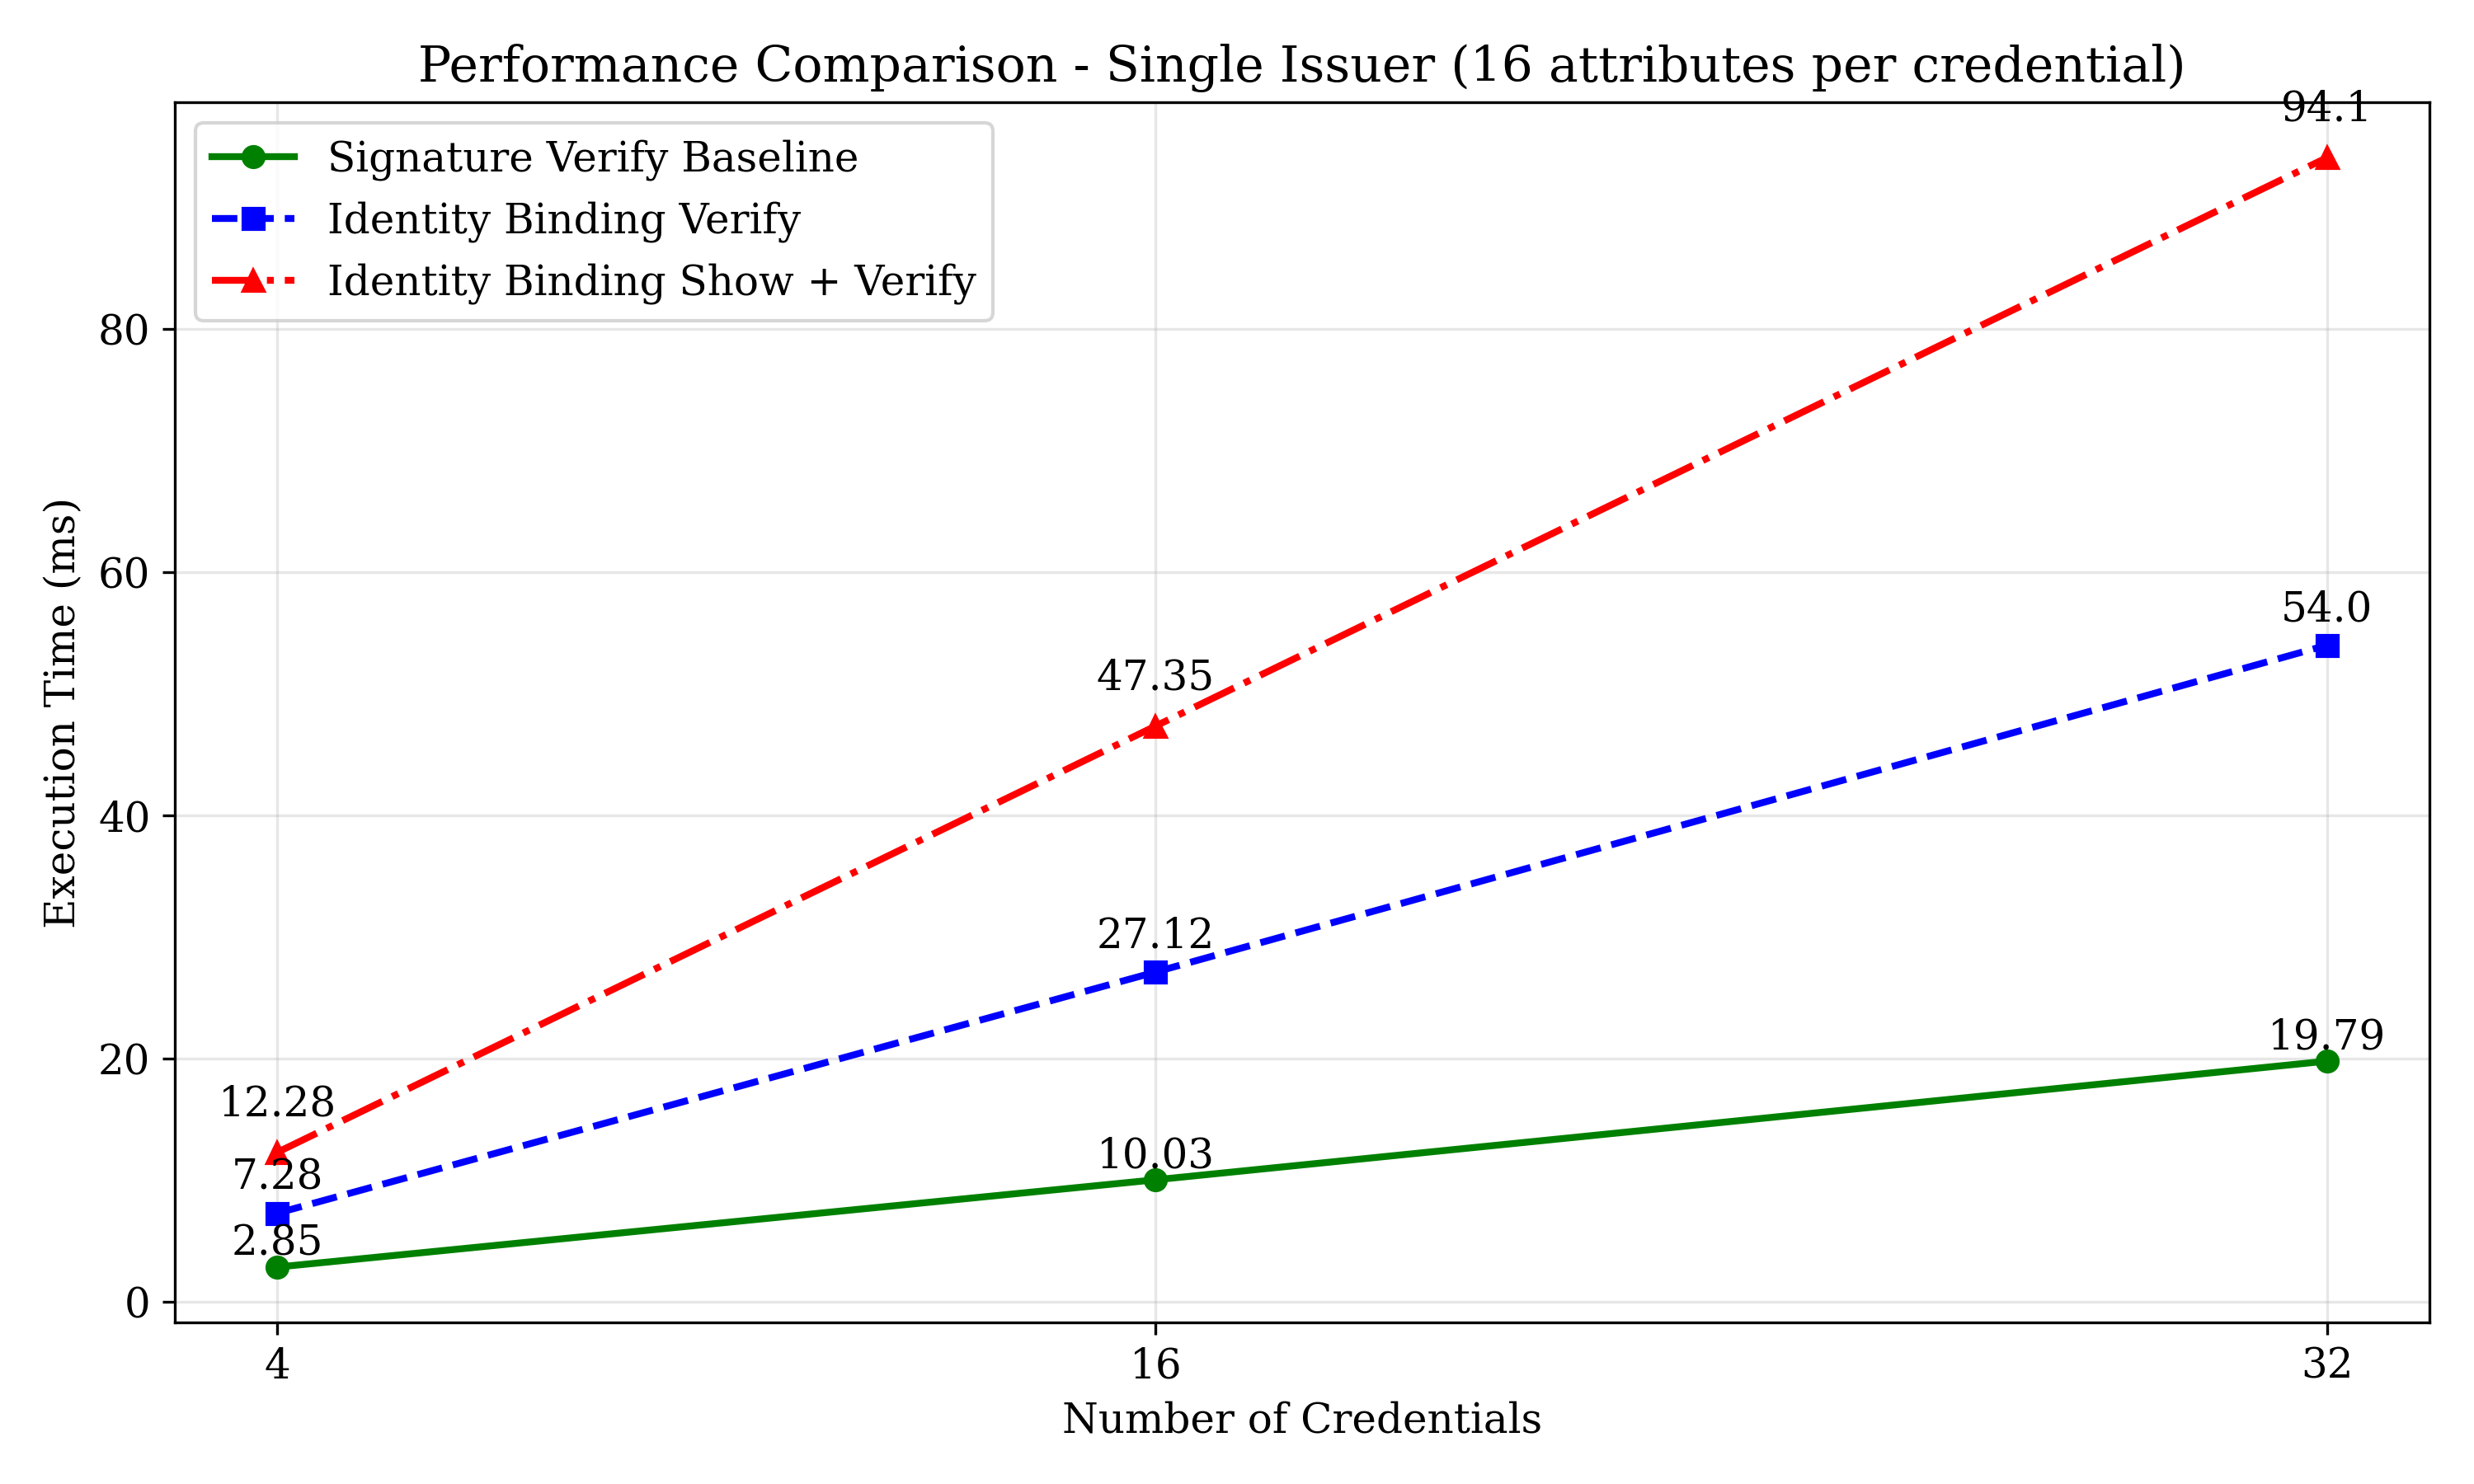
\includegraphics[width=0.48\textwidth]{figures/identity_binding_single_issuer_performance.png}
        \hfill
        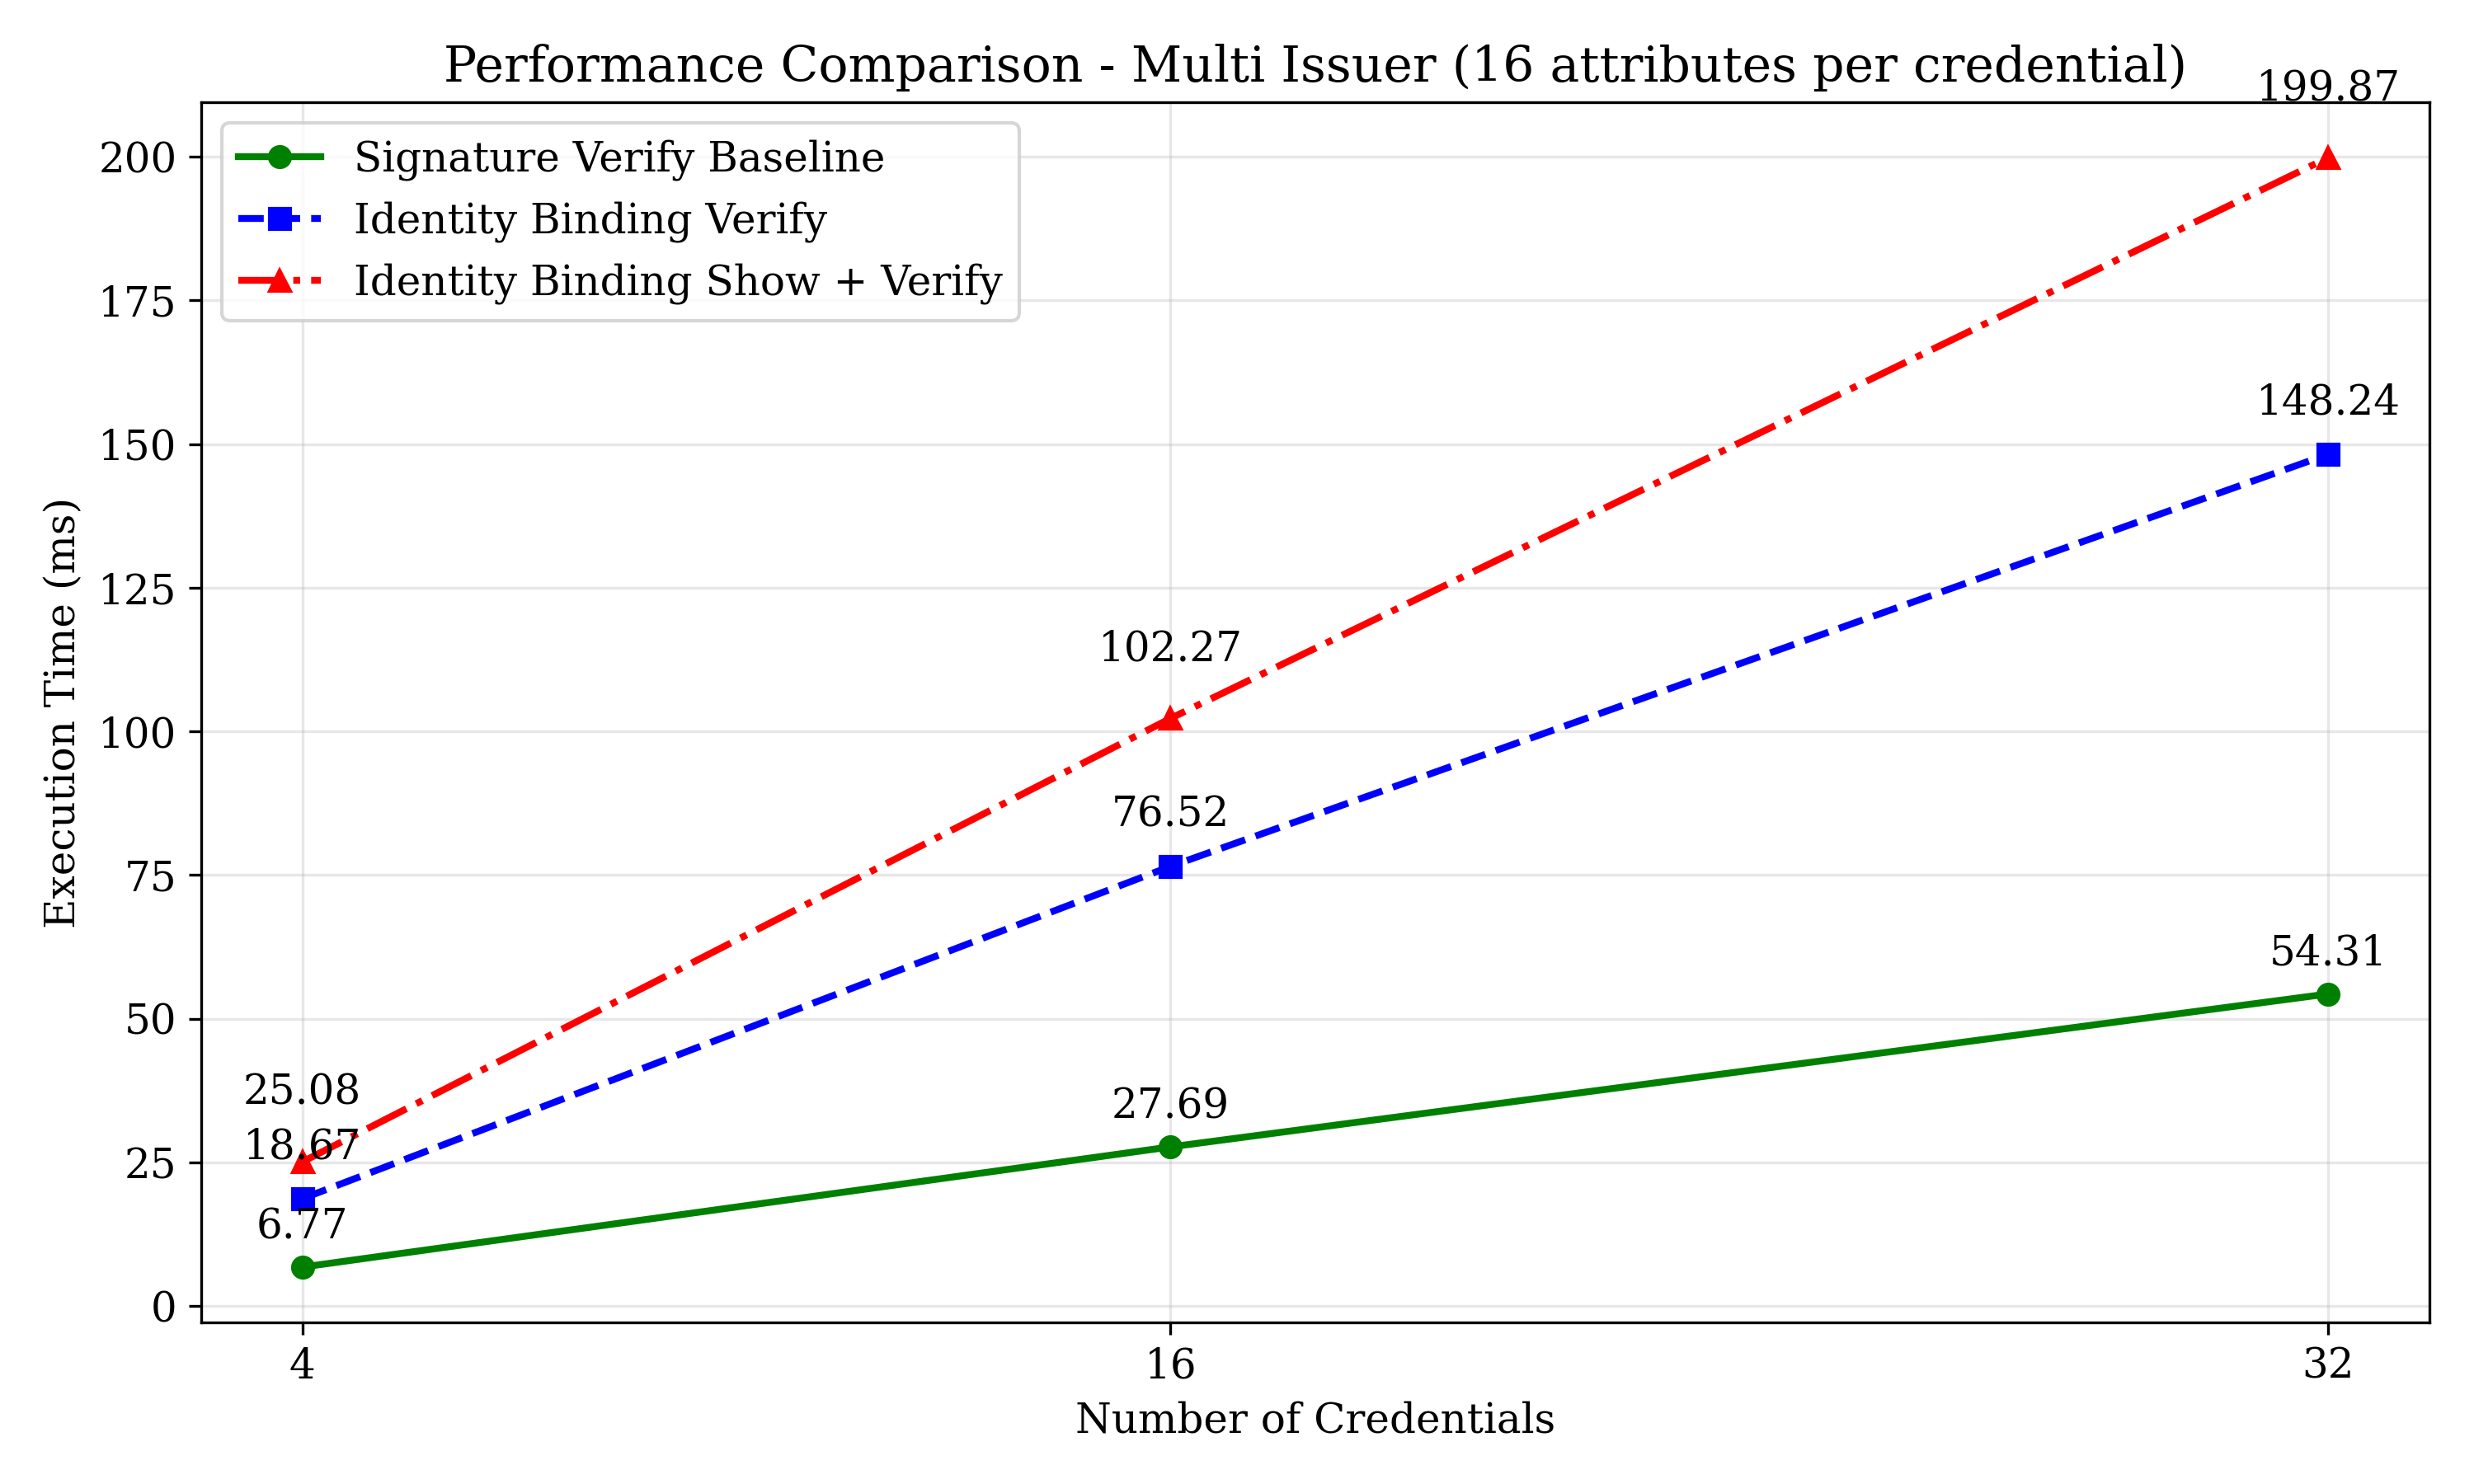
\includegraphics[width=0.48\textwidth]{figures/identity_binding_multi_issuer_performance.png}
    \end{minipage}
    
    \vspace{1em} % Add some vertical space between rows
    
    % Second row with one figure
    \begin{minipage}{\textwidth}
        \centering
        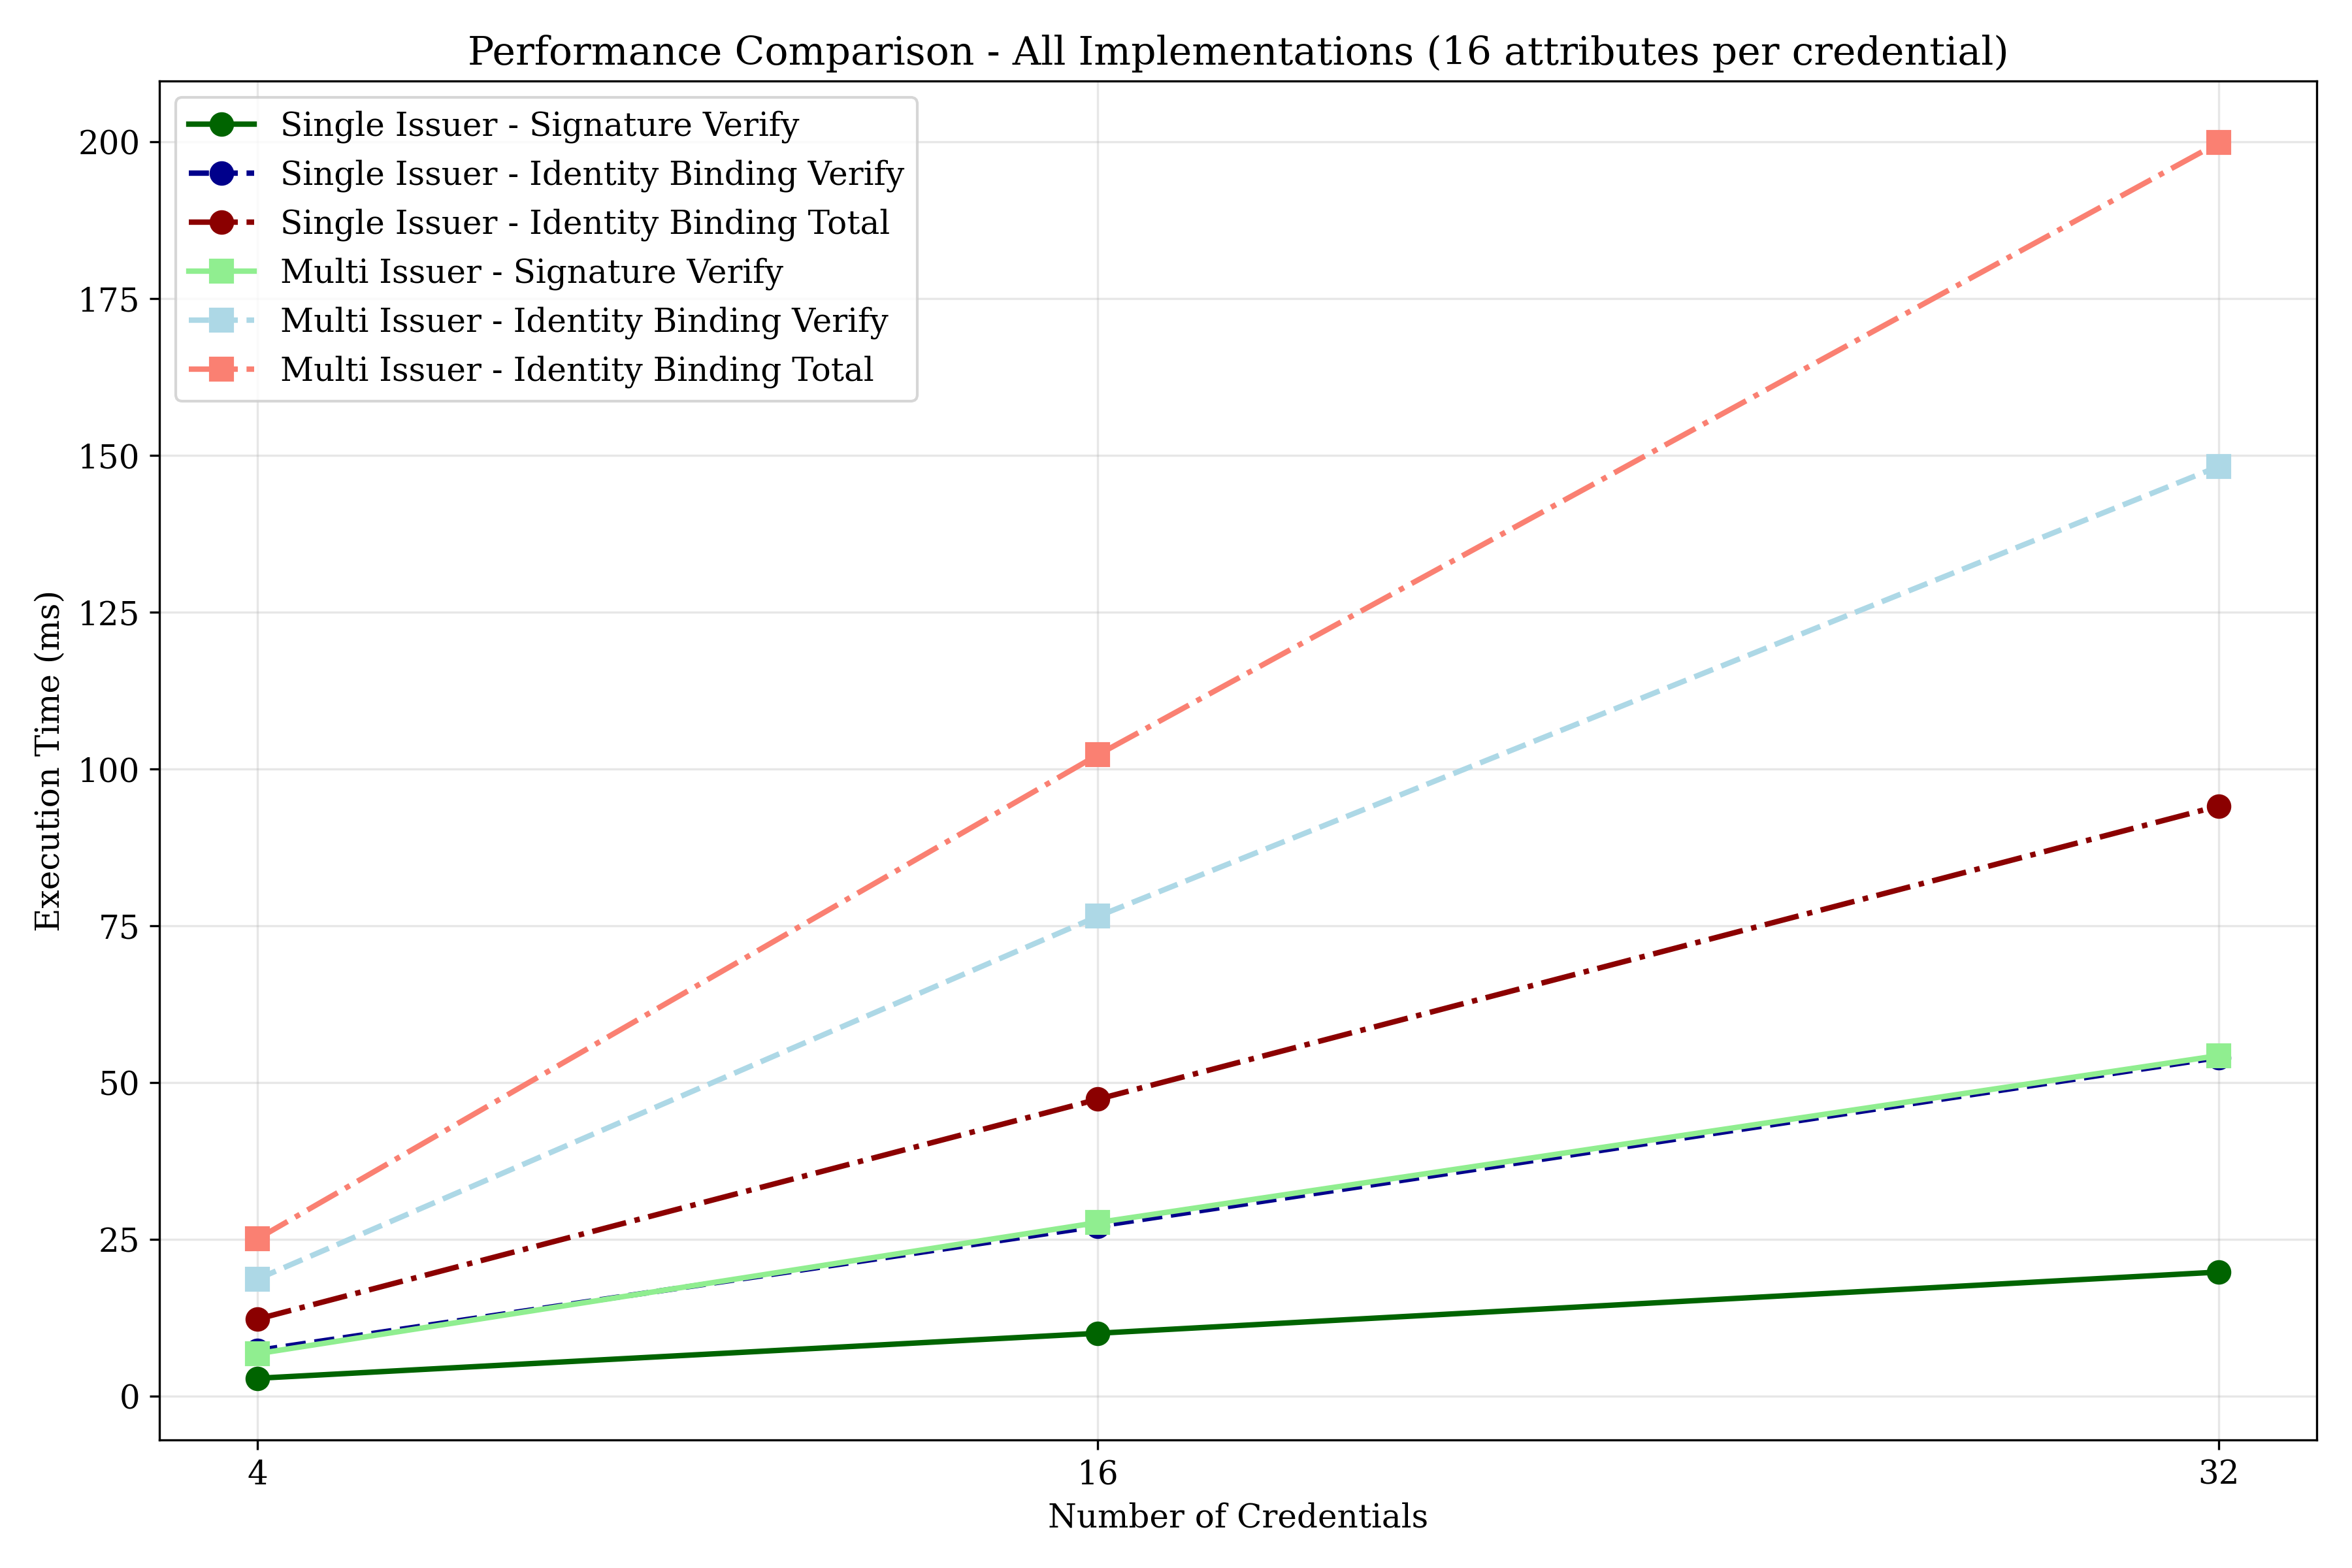
\includegraphics[width=0.48\textwidth]{figures/identity_binding_combined_performance.png}
    \end{minipage}
    
    \caption{Performance comparison between multi-issuer and single-issuer scenarios}
    \label{fig:performance-comparison}
\end{figure}

\clearpage
































\section{Second Attempt}

\newpage
\section{Introduction}
Anonymous credential systems enable users to selectively disclose attributes about themselves while preserving privacy. While significant advances have been made in single-issuer scenarios, modern digital identity ecosystems increasingly require users to present credentials from multiple, mutually distrusting issuers. This chapter addresses the fundamental challenge of how users can privately combine credentials from multiple issuers while proving they belong to the same identity, without revealing that identity.

\subsection{Motivation}
Consider a user who needs to prove they are (1) a resident of a specific jurisdiction from a government-issued ID, (2) employed with sufficient income from an employer credential, and (3) have completed required training from an educational institution. Traditional approaches either compromise privacy by revealing the same identifier across credentials or offer insufficient guarantees that credentials belong to the same individual. Our MIMC-ABC system addresses this gap by providing formal security guarantees for identity binding across credentials from multiple issuers.

\subsection{Contributions}
This chapter makes the following contributions:
\begin{itemize}
    \item Formalization of a security model for multi-issuer credential systems with identity binding
    \item Definition and analysis of the identity binding property for anonymous credentials
    \item Comprehensive attack taxonomy covering credential forgery, predicate manipulation, and identity binding attacks
    \item Security proofs demonstrating how our construction maintains security guarantees as the number of issuers and credentials increases
    \item Performance evaluation methodology comparing private vs. non-private approaches across single and multi-issuer scenarios
\end{itemize}

\section{System Model and Definitions}
\subsection{MIMC-ABC System}
A Multi-Issuer Multi-Credential Attribute-based Anonymous Credential system consists of the following PPT algorithms:

\begin{definition}[MIMC-ABC System]
\begin{itemize}
    \item $\mathsf{Setup}(1^\lambda) \to \mathsf{pp}$: Takes security parameter $\lambda$ in unary, outputs public parameters $\mathsf{pp}$.
    
    \item $\mathsf{OrgKeyGen}(\mathsf{pp}, \ell) \to (\mathsf{osk}, \mathsf{opk})$: Takes public parameters $\mathsf{pp}$ and $\ell$ the upper bound of credential attributes. Outputs organisation's keypair $(\mathsf{osk}, \mathsf{opk})$.
       
    \item $(\mathsf{Obtain}(\vec{m}, \mathsf{opk}, \mathsf{aux}), \mathsf{Issue}(\mathsf{osk}, \mathsf{cm}, \mathsf{aux})) \rightarrow (\mathsf{cred}, \bot)$: An interactive protocol between a user and an issuing organization. The user inputs their message vector $\vec{m} = [\mathsf{id}, \mathsf{ctx}, \mathsf{attrs}]$ containing a unique identifier $\mathsf{id}$ and context $\mathsf{ctx}$. User generates $\mathsf{usk} \stackrel{\$}{\leftarrow} \mathbb{Z}_p$, commits to their messages $\mathsf{cm} \gets \mathsf{CM.Com}(\vec{m}; \mathsf{usk})$. The issuer inputs their secret key $\mathsf{osk}$. The protocol outputs a credential $\mathsf{cred}$ containing $(\sigma, \mathsf{cm})$ to the user and $\bot$ to the issuer.    
    
    \item $(\mathsf{Show}(\{\mathsf{cred}_i\}, \{\mathsf{usk}_i\}, \phi), \mathsf{Verify}(\{\mathsf{cred}_i'\}, \pi)) \rightarrow \{0,1\}$: An interactive protocol between a user and verifier. The user runs $\mathsf{Show}$ with their credentials (signatures and paired commitments), and secret keys. The user rerandomizes their credentials and commitments and computes a proof $\pi$ that satisfies the predicate $\phi$.
    $\mathsf{Verify}$ is run by the verifier, which takes input from the randomized credentials $\mathsf{cred}_i'$, randomized commitments $\mathsf{cm}_i'$, and predicate, proof pair $\phi, \pi$. The protocol outputs 1 if verification succeeds, 0 otherwise.
\end{itemize}
\end{definition}

\subsection{Security Properties}
Our MIMC-ABC system offers three critical security properties:

\begin{itemize}
    \item \textbf{Correctness}: Ensures an honest user with valid credentials can always generate a proof for any predicate their credentials satisfy, which will verify with overwhelming probability.

    \item \textbf{Unforgeability}: Prevents a malicious user, or colluding users, from creating valid proof for new forged credentials, misuse of legitimately issued ones, or unauthorized combination of credentials they don't own.

    \item \textbf{Anonymity}: Protects user privacy, ensuring proofs reveal only that the predicate is satisfied, even if adversaries control the issuers or define predicates.
\end{itemize}

\subsection{Identity Binding Property}
We introduce the identity binding property as a critical component of unforgeability in multi-issuer credential systems:

\begin{definition}[Identity Binding]
A MIMC-ABC system satisfies identity binding if for all PPT adversaries $\mathcal{A}$, there exists a negligible function $\mathsf{negl}$ such that:
\begin{align*}
\Pr\left[\begin{array}{l}
    \mathsf{pp} \gets \mathsf{Setup}(1^\lambda) \\
    \{(\mathsf{osk}_j, \mathsf{opk}_j)\}_j \gets \mathsf{OrgKeyGen}(\mathsf{pp}) \\
    (\{\mathsf{cred}_i'\}, \phi^*, \pi^*) \gets \mathcal{A}^{\mathcal{O}}(\{\mathsf{opk}_j\}_j)
\end{array}
: \begin{array}{l}
    \mathsf{Verify}(\{\mathsf{cred}_i'\}, \phi^*, \pi^*) = 1 \land \\
    \phi^* \text{ requires identity binding} \land \\
    \nexists \mathsf{id} : \forall i, \mathsf{cred}_i \text{ belongs to } \mathsf{id}
\end{array}\right] \leq \mathsf{negl}(\lambda)
\end{align*}
where $\mathcal{O}$ represents the oracles available to the adversary.
\end{definition}

Informally, identity binding ensures that when a predicate requires multiple credentials to belong to the same identity, it is computationally infeasible to produce a valid proof unless all credentials genuinely belong to the same identity.

\section{MIMC-ABC Construction}
Our construction builds upon the foundational primitives established in Chapter 2, specifically leveraging position-binding commitments and rerandomizable signatures.

\subsection{Intuition of Construction}

\subsubsection{Example}
Consider a user holding credentials from three issuers, denoted $j = 1, 2, 3$, each providing one credential $k = 1$. The user rerandomizes each credential’s commitment and signature as follows: $\cm_{j,1}' \gets \CMRand(\cm_{j,1}, \Delta_{r_{j,1}})$ and $\sigma_{j,1}' \gets \RSRand(\sigma_{j,1}, \Delta_{r_{j,1}}, \Delta_{u_{j,1}})$. These rerandomized pairs $(\cm_{j,1}', \sigma_{j,1}')$ are indistinguishable from their original issuance. In the $\Show$ protocol, the verifier confirms their validity: $\RSVer(\sigma_{j,1}', \cm_{j,1}', \vk_j) = 1$ for all $j \in \{1, 2, 3\}$.

\begin{figure}
        \begin{pchstack}[boxed, center, space=4em]
            \begin{pcvstack}
                \procedure[space=auto]{Passport}{%
                \id: 12345, \\
                \ctx: "passport", \\
                \attrs: \mathsf{values}
                }
            \end{pcvstack}
            \pcvspace
            \begin{pcvstack}
                \procedure[space=auto]{Driver License}{%
                 \id: 12345, \\
                \ctx: "dmv", \\
                 \attrs: \mathsf{values}
                }
            \end{pcvstack}
            \pcvspace
            \begin{pcvstack}
                \procedure[space=auto]{University Degree}{%
                 \id: 12345, \\
                \ctx: "usyd{-}bcompsc", \\
                \attrs: \mathsf{values}
                }
            \end{pcvstack}
        \end{pchstack}
    \caption{Three Example Credentials, $\attrs$ holds arbitrary number of attributes such as expiry}
    \label{fig:three-creds}
\end{figure}

Next, the user proves a relation $\mathcal{R}_\phi$ that ensures the credentials satisfy a predicate $\phi$. 
\[
\mathcal{R}_\phi = \left\{ 
\begin{array}{l} 
\forall j, k: \RSVer(\sigma_{j,k}', \cm_{j,k}', \vk_j) = 1 \\ 
\forall j, k: \cm_{j,k}' = \CMRand(\CMCom([\id, \ctx_{j,k}, \attrs_{j,k}]; \usk_{j,k}), \Delta_{r_{j,k}}) \\ 
\phi(\{\ctx_{j,k}, \attrs_{j,k}\}) = 1 
\end{array} 
\right\}
\]

For instance, if $\phi$ requires a valid passport, driver’s license, and university degree, $\mathcal{R}_\phi$ might enforce $\ctx_{1,1} = \text{''passport''}$, $\attrs_{1,1}.\exp > \text{today}$, $\ctx_{2,1} = \text{''dmv''}$, and $\ctx_{3,1} \in \mathcal{D}$ (a set of accredited universities), with all commitments sharing the same $\id$.

\subsection{Sigma-protocol and core relations}

Our MIMC-ABC system relies on five core relations proven via $\Sigma$-protocols:
\begin{enumerate}
  

    \item \textbf{Identity Binding:} For two credentials with commitments $\cm_1$ and $\cm_2$:

    \[
    \rid = \zkpok \left\{ 
    \begin{array}{l} 
    (\cm_1, \cm_2, (\id, \usk_1, \usk_2, \ctx_1, \ctx_2, \attrs_1, \attrs_2)) \\
    \end{array} 
    \middle|
    \begin{array}{l}
    \cm_1 = g^{\usk_1} \cdot g_1^{\id} \cdot g_2^{\ctx_1} \cdot \prod g_i^{\attrs_{1,i}} \wedge \\
     \cm_2 = g^{\usk_2} \cdot g_1^{\id} \cdot g_2^{\ctx_2} \cdot \prod g_i^{\attrs_{2,i}} \\
    \end{array} 
    \right\}
    \]
    
    This proves both credentials share the same $\id$ without revealing the $\id$ value. This generalizes to $n$ credentials by proving equality across all $n$ commitments.
    
    The position-binding property of our commitment scheme (Section \ref{sec:commitment}) ensures this equality relation can't be forged - an adversary can't make two commitments appear to share the same $\id$ when they actually don't.
    
\end{enumerate}

\section{Adversarial Model and Attack Taxonomy}
\label{sec:attack-taxonomy}

We classify potential attacks against MIMC-ABC systems into three categories based on the adversarial goals and security properties being violated:

\subsection{Credential Forgery Attacks}
\begin{itemize}
    \item \textbf{Definition:} Unauthorized creation or modification of credentials
    \item \textbf{Threat model:} External adversaries or corrupt users without legitimate access
    \item \textbf{Security property violated:} Unforgeability of signature scheme
\end{itemize}

\noindent\textbf{Type-1 Forgery (Credential Forgery):} An adversary produces a credential $\mathsf{cred} = (\sigma, \mathsf{cm})$ that verifies without being legitimately issued, breaking the signature scheme's EUF-CMA security.

\begin{example}
An adversary attempts to forge a credential that appears to be issued by a legitimate authority. This attack targets the underlying signature scheme, attempting to create a signature that will verify against the issuer's public key.
\end{example}

\subsection{Predicate Manipulation Attacks}
\begin{itemize}
    \item \textbf{Definition:} Attempts to satisfy unauthorized predicates with legitimate credentials
    \item \textbf{Subtypes:}
    \begin{itemize}
        \item Simple predicate misuse (falsifying a single credential predicate)
        \item Cross-credential predicate manipulation (falsely claiming relationships)
    \end{itemize}
    \item \textbf{Security property violated:} Soundness of zero-knowledge proofs
\end{itemize}

\noindent\textbf{Type-2 Forgery (Predicate Misuse):} A corrupt user with a valid credential for $\mathsf{age} = 17$ attempts to satisfy $\phi = (\mathsf{age} \geq 18)$ by creating a false proof, breaking ZKP soundness.

\begin{example}[Mixed Predicate Misuse]
A corrupt user with a master credential claiming $\mathsf{age} = 25$ and a context credential claiming $\mathsf{drivingClass} = \mathsf{"motorcycle"}$ attempts to satisfy the predicate $\phi = (\mathsf{age} \geq 21 \land \mathsf{drivingClass} = \mathsf{"car"})$ by forging an incorrect zero-knowledge proof.
\end{example}

\subsection{Identity Binding Attacks}
\begin{itemize}
    \item \textbf{Definition:} Breaking the binding between credentials that should share identity
    \item \textbf{Subtypes:}
    \begin{itemize}
        \item Mix-and-match attacks (combining credentials from different identities)
        \item Issuer collusion attacks (issuers collaborating to break binding)
    \end{itemize}
    \item \textbf{Security property violated:} Position-binding of commitment scheme
\end{itemize}

\begin{example}[Credential Binding Attack]
A corrupt user possesses legitimate credentials $\mathsf{cred}_{m,A}$ with $\mathsf{id} = 123$ and $\mathsf{cred}_{c,B}$ with $\mathsf{id} = 456$. They attempt to present these together with a forged zero-knowledge proof $\pi^*$ falsely claiming that both credentials share the same identity.
\end{example}

\begin{example}[Issuer Collusion Attack]
A corrupt user possesses a master credential from issuer $j_1$ with $\mathsf{id} = 123$ and another master credential from issuer $j_2$ with $\mathsf{id} = 456$. The adversary colludes with issuer $j_2$ to create a credential that appears to share the same identity as the credential from $j_1$, attempting to break the identity binding property.
\end{example}

\section{Security Analysis}
\label{sec:security-analysis}

\subsection{Security Scaling Analysis}
We analyze how the security of our MIMC-ABC system scales with increasing numbers of issuers and credentials. Through a reduction to the underlying cryptographic primitives, we show that:

\begin{theorem}
\label{thm:security-scaling}
For a MIMC-ABC system with $n$ issuers and $m$ credentials per user, the probability of an adversary successfully mounting an identity binding attack is bounded by:
\begin{align*}
\mathsf{Adv}^{\mathsf{bind}}_{\mathcal{A}}(\lambda) \leq n \cdot m \cdot \mathsf{Adv}^{\mathsf{pos\text{-}bind}}_{\mathcal{B}}(\lambda) + \varepsilon(\lambda)
\end{align*}
where $\mathsf{Adv}^{\mathsf{pos\text{-}bind}}_{\mathcal{B}}(\lambda)$ represents the advantage against the position-binding property of our commitment scheme, and $\varepsilon(\lambda)$ is a negligible function in the security parameter.
\end{theorem}

\begin{proof}[Proof sketch]
We construct a reduction $\mathcal{B}$ that uses an adversary $\mathcal{A}$ against identity binding to break the position-binding property of our commitment scheme. Given access to oracles for $\mathsf{Obtain}$ and $\mathsf{Show}$, $\mathcal{A}$ outputs credentials $\{\mathsf{cred}_i'\}$, a predicate $\phi^*$ requiring identity binding, and a proof $\pi^*$ that verifies but violates the identity binding property.

Since $\mathcal{A}$ produces a valid proof for credentials with different identities, $\mathcal{B}$ can extract (by the special soundness property of our $\Sigma$-protocols) the witnesses used in generating $\pi^*$. These witnesses must include two different identity values for at least one pair of credentials. 

$\mathcal{B}$ selects a random issuer $j \in [1,n]$ and credential $k \in [1,m]$ and uses the extracted witness to output a position-binding break for the commitment scheme. With probability at least $\frac{1}{n \cdot m}$, this corresponds to the credentials where identity binding was broken.

The full reduction includes careful handling of oracle queries and extraction steps, but this captures the essential security relationship.
\end{proof}

This theorem demonstrates that the security of our identity binding mechanism degrades gracefully as the number of issuers and credentials increases, with only a linear security loss in these parameters.

\subsection{Unforgeability Analysis}
We reduce the unforgeability of our MIMC-ABC system to three underlying properties: EUF-CMA security of the signature scheme, position binding of the commitment scheme, and the soundness of the $\Sigma$-protocol.

\begin{theorem}[Unforgeability]
The MIMC-ABC system is unforgeable if the rerandomizable signature scheme is EUF-CMA secure, the commitment scheme satisfies position binding, and the $\Sigma$-protocol is sound.
\end{theorem}

\begin{proof}[Proof sketch]
We construct a reduction algorithm $\mathcal{B}$ that leverages an adversary $\mathcal{A}$ against MIMC-ABC unforgeability to break one of the underlying security properties.

$\mathcal{B}$ receives a challenge verification key $\mathsf{vk}$ and embeds it in the MIMC-ABC public parameters given to $\mathcal{A}$. For $\mathsf{Obtain}$ queries, $\mathcal{B}$ forwards the commitment to the EUF-CMA signing oracle and returns the signature to $\mathcal{A}$.

When $\mathcal{A}$ outputs a forgery $(\{\mathsf{cred}_i^*\}, \phi^*, \pi^*)$, $\mathcal{B}$ analyzes it according to the following cases:

\begin{enumerate}
    \item \textbf{Case 1:} If any credential in $\{\mathsf{cred}_i^*\}$ contains a signature on a commitment not previously queried, $\mathcal{B}$ outputs this as an EUF-CMA forgery.

    \item \textbf{Case 2:} If all credentials are legitimate but the proof $\pi^*$ demonstrates a predicate $\phi^*$ that the original attributes don't satisfy:
    \begin{itemize}
        \item By the special soundness of the $\Sigma$-protocol, $\mathcal{B}$ extracts a valid witness from $\pi^*$
        \item This witness must include attribute values that satisfy $\phi^*$
        \item Since the original attributes don't satisfy $\phi^*$, the extracted witness must differ from the original commitment opening
        \item This gives two different openings for the same commitment, breaking position binding
    \end{itemize}

    \item \textbf{Case 3:} If the proof $\pi^*$ verifies but neither Case 1 nor Case 2 applies, this directly contradicts the soundness of the $\Sigma$-protocol.
\end{enumerate}

Since any successful forgery falls into one of these categories, and each category leads to breaking an underlying security assumption, the MIMC-ABC system inherits the security of these primitives.
\end{proof}

\subsection{Anonymity Analysis}
\begin{theorem}[Anonymity]
The MIMC-ABC system is anonymous even with malicious issuer keys if the rerandomized signature is computationally indistinguishable from the standard, the commitment scheme is hiding, and the $\Sigma$-protocol is zero-knowledge.
\end{theorem}

\begin{proof}[Proof sketch]
We prove anonymity using a hybrid argument to show the adversary's advantage is negligible:

\begin{description}
    \item[\textbf{Hybrid 0} (Real Game):] The challenger follows the anonymity game exactly. For a randomly chosen $b \in \{0,1\}$, the challenger uses user $i_b$'s credentials to generate $(\mathsf{cred}', \mathsf{cm}', \pi)$ via the real $\mathsf{Show}$ protocol. 
    
    \item[\textbf{Hybrid 1} (Simulated Proof):] The challenger generates $\mathsf{cred}'$ and $\mathsf{cm}'$ by rerandomizing user $i_b$'s credentials, but uses a zero-knowledge simulator $\mathcal{S}$ to produce the proof $\pi$ without using the witness:
    \begin{align*}
        \mathsf{cred}' &\gets \mathsf{RS.Rerand}(\mathsf{cred}_{i_b}, \Delta_r, \Delta_u)\\
        \mathsf{cm}' &\gets \mathsf{CM.Rerand}(\mathsf{cm}_{i_b}, \Delta_r)\\
        \pi &\gets \mathcal{S}(\mathsf{cred}', \mathsf{cm}', \mathsf{opk}, \phi)
    \end{align*}
\end{description}

By the zero-knowledge property of our $\Sigma$-protocol, $\mathsf{Hybrid\:0}$ and $\mathsf{Hybrid\:1}$ are computationally indistinguishable. In $\mathsf{Hybrid\:1}$, the adversary's view is independent of bit $b$ due to:

\begin{enumerate}
    \item The perfect hiding of Pedersen commitments ensures $\mathsf{cm}'$ has a uniform distribution
    \item The rerandomized signature $\mathsf{cred}'$ is computationally indistinguishable from a fresh signature
    \item The simulated proof $\pi$ depends only on public parameters, not on the witness
    \item Our verkey proof mechanism ($\pi_{\mathsf{verkey}}$) ensures issuers cannot embed malicious structures in keys
\end{enumerate}

Therefore, the adversary's total advantage is bounded by the advantage in distinguishing between $\mathsf{Hybrid\:0}$ and $\mathsf{Hybrid\:1}$, which is negligible.
\end{proof}

\section{Performance Evaluation}
We implement our MIMC-ABC system and conduct a comprehensive performance evaluation to quantify the overhead of privacy-preserving identity binding across multiple issuers.

\subsection{Benchmark Methodology}
We evaluate four scenarios:
\begin{enumerate}
    \item \textbf{Non-private Single-Issuer}: Multiple credentials from the same issuer, identity revealed in clear
    \item \textbf{Non-private Multi-Issuer}: Multiple credentials from different issuers, identity revealed in clear
    \item \textbf{Private Single-Issuer}: Multiple credentials from the same issuer with zero-knowledge identity binding
    \item \textbf{Private Multi-Issuer}: Multiple credentials from different issuers with zero-knowledge identity binding
\end{enumerate}

\subsection{Experimental Results}
[Performance evaluation data would be presented here...]

\section{Summary and Future Directions}
This chapter has introduced MIMC-ABC, a multi-issuer multi-credential anonymous credential system with formal identity binding guarantees. We have demonstrated how our system enables users to privately combine credentials from multiple, mutually distrusting issuers while proving they belong to the same identity.

Our security analysis provides formal guarantees that the system remains secure even as the number of issuers and credentials increases, with security reductions to well-established cryptographic assumptions. Our performance evaluation quantifies the overhead of privacy-preserving identity binding and demonstrates the feasibility of our approach for real-world applications.

Future work includes extending the system with hierarchical credential models to enhance accountability while maintaining privacy guarantees, which we will explore in the next chapter.